\chapter{View Handler}
\section{Summary}
Da View Handler Design Pattern hilft beim verwalten aller Views die ein Software System zur Verfügung stellt. Eine View Handler Komponente erlaubt Clients das öffnen, manipulieren und schliessen von Views. Sie koordiniert ausserdem die Abhängigkeiten zwischen Views und organisiert deren Aktualisierung.
\section{Context}
Ein Software System, welches verschiedene Views von Applikations spezifischen Daten anbietet, oder das dass arbeiten mit mehreren Dokumenten unterstützt.
\section{Problem}
Software Systeme die mehrere Views unterstützten benötigen oft zusätzliche Funktionalität für das Verwalten dieser. User wollen Views komfortabel öffnen, manipulieren und schliessen können. Views müssen koordiniert werden, so dass die Änderungen an die anderen weiter propagiert werden. Folgende Forces beeinflussen die Lösung dieses Problems:
\begin{itemize}
	\item Verwalten von mehreren Views soll einfach sein
	\item Implementierungen von verschiedenen Views sollen nicht abhängig von einander sein oder mit dem Code der für die Verwaltung derer Zuständig ist vermischt sein
	\item View Implementationen sollen variieren können und zusätzliche Typen von Views sollen später hinzugefügt werden können.
\end{itemize}
\section{Solution}
Mit dem View Handler Pattern wird das Management der Views vom Rest separiert. Diese View Handler Komponente beinhaltet die Funktionalität fürs öffnen, manipulieren und schliessen von Views. Spezifische Views werden in separaten View Komponenten eingeschlossen, eine für jede Art von View. Suppliers sind für die Lieferung von Daten an die View zuständig. \\
Das View Handler Pattern hat wie das MVC Pattern die Idee den funktionalen Kern von den Views zu trennen. Es gibt allerdings nicht die Gesamtstruktur eines Software Systems vor, sondern gibt nur die Zuständigkeit für die Verwaltung aller Views und ihrer Abhängigkeiten an eine separate Komponente ab. \\
Die View Handler Komponente kann als Abstract Factory und Mediator gesehen werden. Es ist eine Abstract Factory weil Clients unabhängig davon sind, wie spezifisch Views erstellt werden, und es ist ein Mediator weil Clients unabhängig davon sind, wie Views koordiniert werden.
\section{Structure}
Das View Handler Pattern besteht aus vier verschiedenen Komponenten.
\paragraph{View Handler:} Dies ist die Hauptkomponente des Patterns. Sie ist zuständig für das instanzieren, initialisieren, manipulieren, koordinieren und schliessen von Views. Die Hauptaufgabe ist jedoch das bereitstellen von View management Services. Beispiele dafür sind das refreshen von mehreren Views oder das klonen von Views.
\paragraph{Abstract View:} Als Abstract View wird das Interface bezeichnet, welches von allen Views implementiert wird.Der View Handler benutzt dieses Interface für die Erstellung, Koordinierung und das Schliessen von Views. 
\paragraph{Specific View:} Bei der Specific View handelt es sich um die effektiven Implementationen der Abstract Views. Jede Specific View implementiert ihre eigene Display Funktion, welche Daten vom Supplier holt, aufbereitet und dem User anzeigt.
\paragraph{Supplier:} Die Supplier Komponente stellt ein Interface bereit, welches von den Views zur Abfrage und Änderung von Daten benutzt werden kann. Sie benachrichtigt den View Handler bei Änderungen von Daten.
Die folgende Grafik zeigt das Zusammenspiel der Komponenten.
\begin{figure}[H]
	\centering
	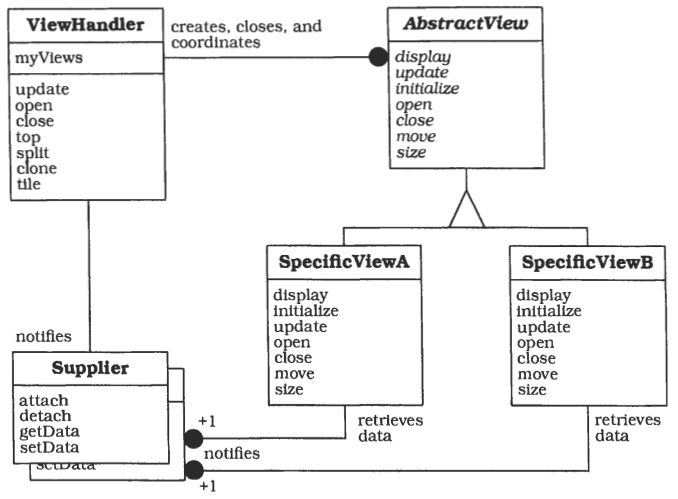
\includegraphics[width=0.6\textwidth]{figures/10-viewhandler-1.png}
	\caption{View Handler Komponenten}
\end{figure}

\section{Variants}
\begin{itemize}
	\item \textit{View Handler with Command Objects:} Diese Variante verwendet Command Objects um den View Handler unabhängig von spezifischen View Interfaces zu halten. Anstatt das die Funktionalität direkt auf der View aufgerufen wird, erstellt der View Handler ein entsprechenden Command und führt diesen aus. Möglich wäre auch das der View Handler den Command an einen Command Processor sendet, welcher diesen dann ausführt.
\end{itemize}

\section{Known Uses}
\begin{itemize}
	\item Macintosh Window Manager
	\item Microsoft Word
\end{itemize}

\section{Consequences}
\begin{itemize}
    \pro{\textbf{Uniform handling of Views}}
    \pro{\textbf{Extensibility and changeability of views}}
    \pro{\textbf{Application specific view coordination}}
    \con{\textbf{Restricted applicability}}
    \con{\textbf{Efficiency}}

\end{itemize}

\section{Relationships}
\begin{itemize}
	\item \textit{Model-View-Controller}
	\item \textit{Presentation-Abstraction-Control}
\end{itemize}

\section{Exam Questions}
\begin{itemize}
  	\item Behauptung:Dies ist eine Behauptung (Lösung: Lösung)
    \item Frage: Dies ist eine Frage? (Lösung)
\end{itemize}
